\documentclass[a4paper,12pt]{article}
\usepackage{amssymb}
\usepackage{amsmath}
\usepackage[utf8]{inputenc} % Umlaute
\usepackage[ngerman]{babel} % Umlaute
\usepackage[T1]{fontenc}    % Umlaute
\usepackage[margin=2.5cm]{geometry}
\usepackage{booktabs}
\usepackage{lmodern}
\usepackage{titlesec}
% Notwendig für Links im Text
\usepackage{hyperref}

% glossar, see http://en.wikibooks.org/wiki/LaTeX/Glossary
% muss NACH hyperref geladen werden, sonst funktionieren die Links nicht
\usepackage[toc]{glossaries}

% Kompatibilität
\ifx\pdftexversion\undefined
\usepackage[dvips]{graphicx}
\else
\usepackage[pdftex]{graphicx}
\DeclareGraphicsRule{*}{mps}{*}{}
\fi

% specify the path to the images
\graphicspath{{bilder/}}

%irgendwas mit section formatierung (titlesec package)
\titleformat{\paragraph}[hang]{\normalfont\normalsize\bfseries}{\theparagraph}{1em}{}
%%%%%%%%%%%%%%%%%%%%%%%%%%%%%%%%%%%%%%%%%%%%%%%%%%%%%%%%%%%%%%%%%%%%%%
% Variablen                                 						 %
%%%%%%%%%%%%%%%%%%%%%%%%%%%%%%%%%%%%%%%%%%%%%%%%%%%%%%%%%%%%%%%%%%%%%%
\newcommand{\authorName}{Tec O'Brain (Entwickler: David Höglinger, Jan Ettrich, Erwin Müller, Benedikt Rittner, Valentin Quapil)}
\newcommand{\auftraggeber}{Karlsruhe Institute of Technology (Teco)}
\newcommand{\auftragnehmer}{\authorName}
\newcommand{\projektName}{Entwurf Earables}
\newcommand{\tags}{\authorName, Architektur, Entwurf, KIT, Informatik, PSE}
\newcommand{\glossarName}{Glossar}
\newcommand{\documentVersion}{0.1}
\title{\projektName}
\date{\today}
\author{Tec O'Brain}

%%%%%%%%%%%%%%%%%%%%%%%%%%%%%%%%%%%%%%%%%%%%%%%%%%%%%%%%%%%%%%%%%%%%%%
% PDF Meta information                                 				 %
%%%%%%%%%%%%%%%%%%%%%%%%%%%%%%%%%%%%%%%%%%%%%%%%%%%%%%%%%%%%%%%%%%%%%%
\hypersetup{
  pdfauthor   = {\authorName},
  pdfkeywords = {\tags},
  pdftitle    = {\projektName)}
}

%%%%%%%%%%%%%%%%%%%%%%%%%%%%%%%%%%%%%%%%%%%%%%%%%%%%%%%%%%%%%%%%%%%%%%
% Create a shorter version for tables. DO NOT CHANGE               	 %
%%%%%%%%%%%%%%%%%%%%%%%%%%%%%%%%%%%%%%%%%%%%%%%%%%%%%%%%%%%%%%%%%%%%%%
\newcommand\addrow[2]{#1 &#2\\ }

\newcommand\addheading[2]{#1 &#2\\ \hline}
\newcommand\tabularhead{\begin{tabular}{lp{13cm}}
\hline
}

\newcommand\addmulrow[2]{ \begin{minipage}[t][][t]{2.5cm}#1\end{minipage}%
   &\begin{minipage}[t][][t]{8cm}
    \begin{enumerate} #2   \end{enumerate}
    \end{minipage}\\ }

\newenvironment{usecase}{\tabularhead}
{\hline\end{tabular}}

\usepackage{microtype}
%%%%%%%%%%%%%%%%%%%%%%%%%%%%%%%%%%%%%%%%%%%%%%%%%%%%%%%%%%%%%%%%%%%%%%
% GLOSSARY ENTRIES                 	                              	 %
%%%%%%%%%%%%%%%%%%%%%%%%%%%%%%%%%%%%%%%%%%%%%%%%%%%%%%%%%%%%%%%%%%%%%%
\newglossaryentry{Datenbank}{name={Datenbank},
	description={Die Datenbank speichert die Trainingsdaten in Form von DBEntries. Dabei wird die Datenbank von dem Plugin SQLite benutzt.}}
\newglossaryentry{CSV}{name={CSV},
	description={CSV steht für "Comma-Seperated-Value" ein Dateityp, bei dem die Attribute durch ein Komma getrennt werden. Eine Zeile bildet dabei immer einen Eintrag ab. Das Format ist human-readable und veränderbar.}}
\makeglossaries
\loadglsentries{Glossar.tex}

%%%%%%%%%%%%%%%%%%%%%%%%%%%%%%%%%%%%%%%%%%%%%%%%%%%%%%%%%%%%%%%%%%%%%%
% THE DOCUMENT BEGINS             	                              	 %
%%%%%%%%%%%%%%%%%%%%%%%%%%%%%%%%%%%%%%%%%%%%%%%%%%%%%%%%%%%%%%%%%%%%%%
\begin{document}
\pagenumbering{roman}
 \begin{titlepage}
\maketitle
\thispagestyle{empty} % no page number

\begin{verbatim}












\end{verbatim}


  \begin{tabular}[t]{p{4 cm}p{8 cm}}
	Projekt:       & \projektName \\[1.2ex]
	Auftraggeber:  & \auftraggeber\\[1.2ex]
	Auftragnehmer: & \auftragnehmer\\[1.2ex]
  \end{tabular}


\begin{tabular}[t]{|p{4 cm}|p{8 cm}|}
\hline
\textbf{Datum} & \textbf{Autor(en)} \\
\hline
\hline
\today & \authorName \\
\hline
\end{tabular}
\end{titlepage}
         % Deckblatt.tex laden und einfügen
 \setcounter{page}{2}
 \tableofcontents          % Inhaltsverzeichnis ausgeben
 \clearpage
 \pagenumbering{arabic}
%%%%%%%%%%%%%%%%%%%%%%%%%%%%%%%%%%%%%%% CONTENT %%%%%%%%%%%%%%%%%%%%%%%%%%%%%%%%%%%%%%%%%%%%%%%

\section{Einleitung}
In diesem Dokument wird der Entwurf der \Gls{CPB}, des Erweiterungsmoduls und der App spezifiziert. Es wird auf die jeweiligen Klassen eingegangen und ihre Funktion erläutert. Außerdem wird die Interaktion der einzelnen Komponenten, mit Hilfe von Sequenzdiagrammen, beschrieben.

\section{Aufbau}
	\subsection{Architekturdiagramm}
	\begin{center}
		\vspace{100px}
		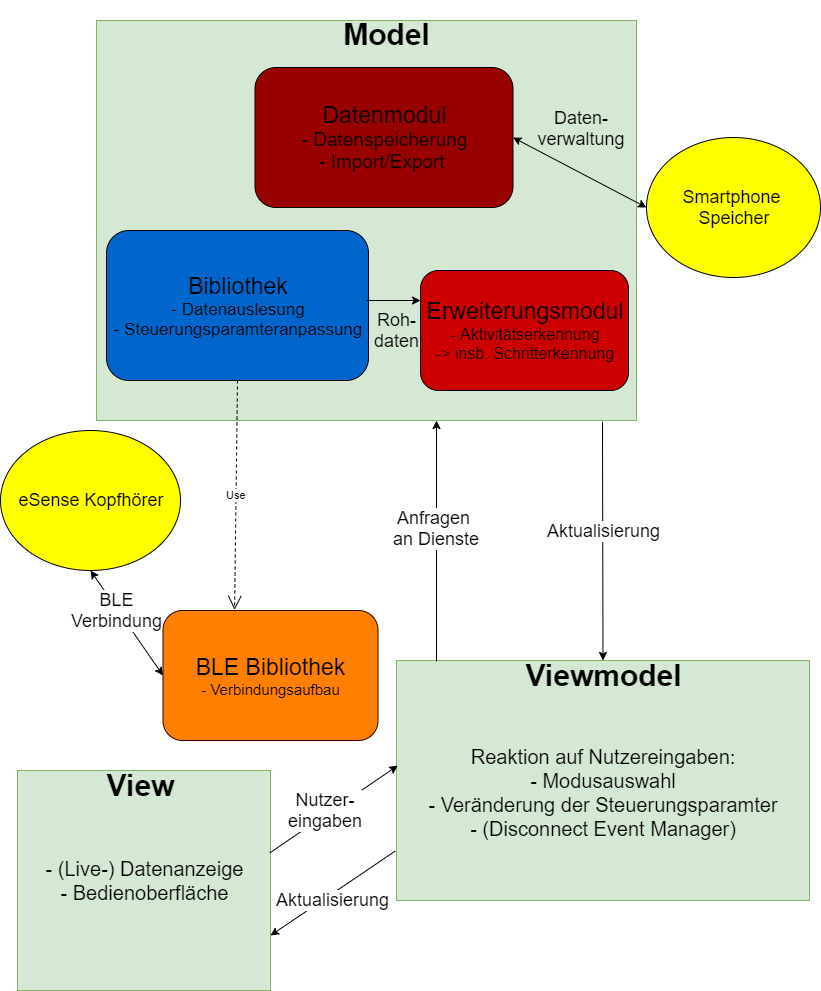
\includegraphics[width=0.8\textwidth]{./Diagramme/Achi5.png}
	\end{center}
	\clearpage %%sieht sonst noch zerrissener aus;    Gehts nicht irgendwie schöner? Sodass das Diagramm ganz oben quasi anliegt?
	\subsection{Kurze Erläuterung zum Architekturdiagramm}
  Wir haben uns bei der Architekturdiagramm für \textsf{Model-View-Viewmodel}, eine Spezialisierung  des Entwurfsmusters Model-View-Controller, entschieden.
  Dabei gibt es folgende Komponenten:
  \begin{itemize}
    \item \textsf{\glqq View\grqq{}} enthält alle grafisch angezeigten Elemente, also die Datenanzeige und Bedienoberfläche der App.
    \item {\textsf{\glqq Model\grqq{}} enthält die Geschäftslogik der App und ist stark nach außen abgekapselt. In diesen Bereich fallen die meisten komplexen Teile der App, die als Dienste (Services) vom Viewmodel aus verwaltet werden sollen. Wesentlich sind dabei (vollständige Angabe im Entwurf): \begin{itemize}
      \item Die Verwaltung der anfallenden Produktdaten (Abruf und Bereitstellung der gespeicherten Daten in der Datenbank, im CSV-Format) über ein Datenmodul
      \item Die Bibliothek, die für die Kommunikation mit den \Gls{Earables} (Verbindungsaufbau, Start und Stopp des Samplings, Konfiguration der \Gls{Steuerungsparameter}, Auslesen der Sensordaten) zuständig ist. Dazu wird eine externe Bibliothek\footnote{https://github.com/xabre/xamarin-bluetooth-le} verwendet.
      \item Das Erweiterungsmodul, das sich um die Aktivitätserkennung kümmert. Dieses nutzt dabei die Schnittstellen der Bibliothek.
    \end{itemize}
    Die Services sind dabei jeweils unabhängig vom restlichen Model funktionsfähig und dadurch leichter testbar.}
    \item \textsf{\glqq Viewmodel\grqq{}} ist das Bindeglied zwischen View und Model. Es enthält die Logik der UI, wird also bei Benutzerinteraktion vom View aufgerufen. Es gibt dann die entsprechenden Anweisungen an das Model weiter. Darüber hinaus kümmert es sich darum, dass in bestimmten Fällen die Anzeige der App angepasst wird, zum Beispiel bei Verbindungsabbruch zu den \Gls{Earables}. 
    
  \end{itemize}
  Der Vorteil dieser Architektur ist eine klare Trennung von Benutzerinteraktion und Programmlogik sowie eine lose Kopplung zwischen einzelnen Funktionalitäten, was die Flexibilität und das modulare Testen deutlich erleichtert.
\clearpage
  \subsection{Klassendiagramm}
hier kommt ein mal das Klassendiagramm rein mit Verweis auf den Anhang - valle
\clearpage
%%\section{Klassenübersicht} brauchen wir nicht, da das bei uns schon alles im Inhaltsverzeichnis aufgelistet wird.
\section{Klassenbeschreibung Model}
\subsection{Bibliothek}
\subsubsection{BibMain}

\paragraph{Klassenbeschreibung:}
Diese Klasse ist das Herz der Bibliothek. Sie besitzt alle Schnittstellen, über die später kommuniziert werden kann. Um eine BLE Verbindung herzustellen benutzt sie das Bluetooth LE Plugin for Xamarin.

\paragraph{Attribute:}
\begin{itemize}
	\item[+] \textbf{imuDataRecived: EventHandler<DataEventArgs>}\\Das Attribut IMUDataRecieved ist vom Typ IMUDataRecivedEventHandler und beinhaltet die IMU Daten eines Eintrags und die Configration der Earables.
	\item[+] \textbf{buttonPressed: EventHandler <ButtonEventArgs>}\\ Das Attribut buttonPressed ist vom Typ PuttonPressedEventHandler und wird benötigt um das drücken des Knopfes an den Earables weiterzuleiten.
	\item[+] \textbf{deviceConnectionStateChanged: EventHandler<DeviceEventArgs>}\\ Das Attribut divceConnectionStateChanged ist vom \\Typ deviceConnectionStateChangedEventHandler und wird benötigt um den aktuellen Verbindungsstatus weiterzuleiten.
	\item[+] \textbf{configuration: ConfigContainer}\\ In diesem Attribut befinden sich die Configurationsvariablen für die Earables.
	\item[+] \textbf{characteristcs: Characteristics}\\ Das Attribut beinhaltet allle Charakteristiken.
\end{itemize}

\paragraph{Methoden:}
\begin{itemize}
	\item[+] \textbf{<constructor>BibMain()}\\ Im Construktor werden die Atribute ble und adapter initialisiert.
	\item[+] \textbf{startScanning(): DeviceList<List>}\\ Diese Methode legt eine neue Liste vom Typ Idivice an, in der sie alle gefundenen Devices speichert und anschließend zurückgibt. Sie benutzt die Mehode DeviceDiscoverd und StartScanningForDevicesAsync aus dem Interface Iadapter und die Methode.
	\item[+] \textbf{connectToDevice(device: Idevice): Boolean}\\ Mit dieser Methode kann sich der Nutzter mit einem Bluetoothgerät verbinden. Er wählt in der Liste  ein Device aus und übergibt es als Parameter. Falls die Verbindung erfolgreich war wird true zurückgegeben. Konnte keine Verbindung hergestellt werden wird false zurückgegeben. Hierbei wird die Methode ConnectToDeviceAsync aus dem BLE\_Pugin der Klasse IAdapter zur Hilfe genommen. Zusätzlich werden gleich alle benötigten Charakteristiken geladen und abgespeichert um sie nicht immer neu laden zu müssen wenn sie gebracuht werden. Das geschieht mit Hilfe der Methoden GetServicesAsync und GetCharacteristicAsync aus dem BLE\_Plugin.
	\item[+] \textbf{disconnectFromDevice(): Boolean}\\ Falls man eine Verbindung zu einem Device besitzt wird diese getrennt und es wid true zurückgegeben. Wenn man keine Verbindung besitzt passiert nichts und es wird false zurückgegeben. Zum Trennen der Verbindung wird die Methode DisconnectDeviceAsync aus dem BLE\_Pugin der Klasse Iadapter benutzt.
	\item[+] \textbf{startSampling(): Boolean}\\ Diese Methode startet die Datenaufzeichnung des IMU. Falls die Datenaufzeichnung erfoglreich gestartet wurde wird true zurückgegeben, ansonsten false. Die Methode WriteAsync aus dem BLE\_Plugin ermöglicht es die charakteristik zu beschreiben. Hinweis: Ist die Samplingrate nicht gesetzt, wird die Standarteinstellung genommen.
	\item[+] \textbf{stopSampling(): Boolean}\\Die Datenaufzeichnung des IMU wird mit dieser Methode gestoppt. Falls die Datenaufzeichnung erfoglreich gestoppt wurde wird true zurückgegeben, ansonsten false. Die Methode WriteAsync aus dem BLE\_Plugin ermöglicht es die charakteristik zu beschreiben.
	\item[+] \textbf{setSampligrate(heart int): Boolean}\\Die Samplingrate wird gesetzt und gespeichert. Bei erfolgreichem sezten wird true zurückgegeben ansonsten false. Die Methode WriteAsync aus dem BLE\_Plugin ermöglicht es die charakteristik zu beschreiben.
	\item[+] \textbf{setLowPassFilterAccelerometer(accelerometerLPF LPF\_Accelerometer): Boolean}\\ Im Konstruktor werden die Attribute ble und adapter initialisiert.
	\item[+] \textbf{getLowPassFilterAccelerometer(): LPF\_Accelerometer}\\ Im Construktor werden die Atribute ble und adapter initialisiert.
	\item[+] \textbf{setLowPassFilterGyroscope(gyroscopeLPF LPF\_Gyroscope): Boolean}\\ Mit dieser Methode wird der Low Pass Filter des Gyroscops gesezt. Bei erfolgreichem sezten wird true zurückgegeben ansonsten false. Bei dem Übergabeparameter hadelt es sich um ein Enum, der angibt auf welchen Wert der Low Pass Filter gesetzt werden soll. Die Methode WriteAsync aus dem BLE\_Plugin ermöglicht es die charakteristik zu beschreiben.
	\item[+] \textbf{getLowPassFilterGyroscope(): LPF\_Gyroscope}\\Die Methode gibt an auf was der LPF des Gyroscops momentan gesetzt ist. Er wird in Form des LPF\_Accelerometer Enums zurückgegeben. 
	\item[+] \textbf{getBatteryVoltage(): int}\\ getBatteryVoltage gibt die voltanzahl der Batterie zurück. Die Methode ReadAsync aus dem BLE\_Plugin ermöglicht es die charakteristik zu lesen.
	\item[+] \textbf{onIMUDataRecived(): void}\\Falls neue IMU-Daten vorliegen wird diese Methode aufgerufen und benachrichtigt alle Listener des Events IMUDataRecieved, dass neue Daten anliegen.
	\item[+] \textbf{onPushButtonPressed(): void}\\ Falls der Knopf an den Earables gedrückt wurde wird diese Methode aufgerufen und benachrichtigt alle Listener des Events buttonPressed, dass der Knopf gedrückt wurde.
	\item[+] \textbf{onDeviceConnected(): void}\\ Falls eine Verbindung mit einem Device hergestellt wurde oder eine besthenden Verbindung aufgelößt wurde wird diese Methode aufgerufen und benachrichtigt alle Listener des Events deviceConnectionStateChanged, dass sich dert Verbindungsstatus geändert hat.
\end{itemize}


\subsubsection{Constants}
\paragraph{Klassenbeschreibung:}
Die Constants Klasse enthält alle Konstanten, die benötigt werden um die entsprechenden Service, Descriptoren und Charakteristiken aus den Earables zu lesen. Sie ist als static gekennzeichnet da es keinen Sinn macht sie zu instanzieren weil sie nur Konstanten bereitstellt.

\paragraph{Attribute:}
\begin{itemize}
	\item[+] \textbf{START/STOP\_IMU\_SAMPLIG\_CHAR: String}\\Dieser String enthält die Beschreibung der Charakteristik um das IMU Daten Sampling zu starten und zu stoppen.
	\item[+] \textbf{SENSORDATA\_CHAR: String}\\Dieser String enthält die Beschreibung der Charakteristik in dem die IMU Sensordaten gespeichert werden.
	\item[+] \textbf{PUSHBUTTON\_CHAR: String}\\Dieser String enthält die Beschreibung der Charakteristik in dem der Push Button Status gespeichet wird.
	\item[+] \textbf{BATTERY\_CHAR: String}\\Dieser String enthält die Beschreibung der Charakteristik in dem die Batterieladung gespeichert wird.
	\item[+] \textbf{ACCELEROMETER\_GYROSCOPE\_LPF\_CHAR: String}\\Dieser String enthält die Beschreibung der Charakteristik in um den Low Pass Filter für den Accelerometer und das Gyroscope zu setzen.
	\item[+] \textbf{NOTIFICATION\_DESCRIPTOR: String}\\Dieser String enthält die Beschreibung des Descriptors um die benachrichtigung über neue IMU Sensordaten oder den Push Button Status ein und aus zu schalten.
\item[+] \textbf{ACCES\_SERVICE: String}\\Dieser String enthält die Beschreibung des Services Acces-service, der die meisen charakteristiken bereitstellt.
\item[+] \textbf{NOCH\_EIN\_SERVICE\_SERVICE: String}\\Muss noch rausfinden welche charakteristiken dieser service bereit stellt.
\end{itemize}


\subsubsection{LPF\_Gyroscope}
Dieses Enum beinhaltet alle möglichen Low Pass Filter Werte, die der LPF für das Gyroscope annehmen kann.

\paragraph{Attribute:}
\begin{itemize}
	\item \textbf{250Hz}\\Steht dafür, dass der LPF 250 Hz annehmen kann.
	\item \textbf{184Hz}\\Steht dafür, dass der LPF 184 Hz annehmen kann.
	\item \textbf{92Hz}\\Steht dafür, dass der LPF 92 Hz annehmen kann.
	\item \textbf{41Hz}\\Steht dafür, dass der LPF 41 Hz annehmen kann.
	\item \textbf{20Hz}\\Steht dafür, dass der LPF 20 Hz annehmen kann.
	\item \textbf{10Hz}\\Steht dafür, dass der LPF 10 Hz annehmen kann.
	\item \textbf{5Hz}\\Steht dafür, dass der LPF 5 Hz annehmen kann.
	\item \textbf{3600Hz}\\Steht dafür, dass der LPF 3600 Hz annehmen kann.
	\item \textbf{OFF}\\Steht dafür, dass der LPF aus ist.
\end{itemize}


\subsubsection{LPF\_Accelerometer}
Dieses Enum beinhaltet alle möglichen Low Pass Filter Werte, die der LPF für das Accelerometer annehmen kann.

\paragraph{Attribute:}
\begin{itemize}
	\item \textbf{460Hz}\\Steht dafür, dass der LPF 460 Hz annehmen kann.
	\item \textbf{184Hz}\\Steht dafür, dass der LPF 184 Hz annehmen kann.
	\item \textbf{92Hz}\\Steht dafür, dass der LPF 92 Hz annehmen kann.
	\item \textbf{41Hz}\\Steht dafür, dass der LPF 41 Hz annehmen kann.
	\item \textbf{20Hz}\\Steht dafür, dass der LPF 20 Hz annehmen kann.
	\item \textbf{10Hz}\\Steht dafür, dass der LPF 10 Hz annehmen kann.
	\item \textbf{5Hz}\\Steht dafür, dass der LPF 5 Hz annehmen kann.
	\item \textbf{OFF}\\Steht dafür, dass der LPF aus ist.
\end{itemize}


\subsubsection{ConfigContainer}
Diese Klasse beinhaltet alle Einstellungsmöglichkeiten für die Earables.

\paragraph{Attribute:}
\begin{itemize}
	\item[+] \textbf{samplerate: int}\\Hier wird die Samplerate gespeichert, in der die Earables neue Daten des IMU aufzeichnen.
	\item[+] \textbf{gyroscopeLPF: LPF\_Gyroscope}\\Dieses Attribut enthält den aktuell eingestellten LPF für das Gyroscope.
	\item[+] \textbf{accelerometerLPF: LPF\_Accelerometer}\\Dieses Attribut enthält den aktuell eingestellten LPF für den Accelerometer.
\end{itemize}


\subsubsection{IMUDataExtractor}
Diese Klasse Übernimmt das Umwandeln des Bit Strings in verschiedene Einheiten.
Die Klasse wurde erstellt um der BibMan Klasse arbeit abzunehmen und Logik zu entkopel, so dass sich die BibMain Klasse nur um die Kommunikation mit den Earables kümmern muss. Sie ist static da es keinen Sinn macht sie zu instanziieren weil sie nur einen Dienst anbietet.

\paragraph{Methoden:}
\begin{itemize}
	\item[+] \textbf{extractIMUDataString(byteString: int, accScaleFactor: int, GyroScaleFactor): IMUDataEntry}\\Diese Methode erstellt aus der übergebenen Bitfolge ein IMUDataEntry, indem sie die Informationen aus dem BytSring auswertet und in verschiedene Einheiten umrechnet. Zum umrechnen benötigt sie noch den accScaleFactor und den gyroScaleFactor. Sie erzeugt ein neues IMUDataEntry Objekt und gibt es als Rückgabewert zurück.
\end{itemize}


\subsubsection{IMUDataEntry}
Diese Klasse besitzt alle ausgewerteten Informationen, die in einem „Packet“ von den Earables ankommen.

\paragraph{Attribute:}
\begin{itemize}
	\item[+] \textbf{gyroscope: Gyroscope}\\In diesem Attribut sind die gemessenen Werte des Gyroscopes enthalten.
	\item[+] \textbf{accelerometer: Accelerometer}\\In diesem Attribut sind die gemessenen Werte des Accelerometerss enthalten.
\end{itemize}


\subsubsection{Gyroscope}
Diese Klasse besitzt alle ausgewerteten Gyroscopedaten.

\paragraph{Attribute:}
\begin{itemize}
	\item[+] \textbf{deg/s\_X: float}\\Gibt an um wie viel Grad pro Sekunde sie die Earables in X Richtung gedreht haben.
	\item[+] \textbf{deg/s\_Y: float}\\Gibt an um wie viel Grad pro Sekunde sie die Earables in Y Richtung gedreht haben.
	\item[+] \textbf{deg/s\_Z: float}\\Gibt an um wie viel Grad pro Sekunde sie die Earables in Z Richtung gedreht haben.
\end{itemize}


\subsubsection{Accelerometer}
Diese Klasse besitzt alle ausgewerteten Accelerometer Daten.

\paragraph{Attribute:}
\begin{itemize}
	\item[+] \textbf{m/s\^2\_X: float}\\Gibt an um wie viel Meter pro\ Sekunde\^2 sich die Earables in X Richtung beschleunigt haben.
	\item[+] \textbf{m/s\^2\_Y: float}\\Gibt an um wie viel Meter pro Sekunde \^2 sich die Earables in Y Richtung beschleunigt haben.
	\item[+] \textbf{m/s\^2\_Z: float}\\Gibt an um wie viel Meter pro Sekunde \^2 sich die Earables in Z Richtung beschleunigt haben.
	\item[+] \textbf{g\_X: float}\\Gibt an um wie viel G sich die Earables in X Richtung beschleunigt haben.
	\item[+] \textbf{g\_Y: float}\\Gibt an um wie viel G sich die Earables in Y Richtung beschleunigt haben.
	\item[+] \textbf{g\_Z: float}\\Gibt an um wie viel G sich die Earables in Z Richtung beschleunigt haben.
\end{itemize}


\subsubsection{Characteristics}
In dieser Klasse werden die Charkterisiken gespeichert um sie nicht jedes mal neu zu laden falls sie gebraucht werden.

\paragraph{Attribute:}
\begin{itemize}
	\item[+] \textbf{start/stopIMUSamplingChar: ICharacteistic}\\Speichert die Charakteristik um das IMU sampling zu starten oder zu stoppen.
	\item[+] \textbf{sensordata: ICharacteisticChar}\\Speichert die Charakteristik in der die Sensordaten liegen.
	\item[+] \textbf{pushbutton: ICharacteisticChar}\\Speichert die Charakteristik in der der Status des Push Button gespeichert wird.
	\item[+] \textbf{battery: ICharacteisticChar}\\Speichert die Charakteristik in der die verbleibende Battrieladung gespeichert wird.
	\item[+] \textbf{AccelerometerGyroscopeLPFChar: ICharacteistic}\\Speichert die Charakteristik in der die Konfiguration des LPF für den Accelerometer und das Gyroscope geschrieben wird.
\end{itemize}


\subsubsection{DeviceEventArgs}
Dieses Event benachrichtigt Listener, falls sich der Verbindungsstatus seines Devices ändert.
%%?? valle: schreiben wir jetzt gar nicht mehr Klassenbeschreibung drüber?
%%valle: das ist doch kein Event! 
\paragraph{Attribute:}
\begin{itemize}
	\item[+] \textbf{connected: Boolean}\\Ist true falls eine BLE Verbindung mit einem Device existiert und false falls nicht.
	\item[+] \textbf{deviceName: String}\\Beinhaltet den Devicenamen des Devices, mit dem der Nutzer verbunden ist. %%bitte deutsch
\end{itemize}

\paragraph{Methoden:}
\begin{itemize}
	\item[+] \textbf{<constructor>DeviceEventArgs(connected: Boolean, deviceName: String): void}\\Zusätzlicher Konstruktor um die Attribute setzten zu können
\end{itemize}


\subsubsection{ButtonEventArgs}
Dieses Event benachrichtigt Listener, falls der Knopf der Earables gedrückt wurde.


\subsubsection{DataEventArgs}
Dieses Event benachrichtigt Listener, falls der neue IMU Daten vorliegen.

\paragraph{Attribute:}
\begin{itemize}
	\item[+] \textbf{data: IMUDataEntry}\\Hier handelt es sich um die aktuellen IMU Datenaufzeichnung.
	\item[+] \textbf{configs: ConfigContainer}\\Hier werden die aktuellen configurationen gespeichert.
\end{itemize}

\paragraph{Methoden:}
\begin{itemize}
	\item[+] \textbf{<constructor>DataEventArgs(connected: Boolean, deviceName: String): void}\\Zusätzlicher Konstruktor um die Attribute setzten zu können
\end{itemize}






\subsection{Erweiterungsmodul}
	\subsubsection{IManager}
	
	\subsubsection{IActivityManager}
	\subsubsection{ActivityManager}
	
	\subsubsection{Activity}
	
	\subsubsection{AbstractSitUpActivity}
	\subsubsection{SitUpActivityThreshold}
	
	\subsubsection{AbstractStepActivity}
	\subsubsection{StepActivityActivityThreshold}
	
	\subsubsection{AbstractRunningActivity}
	\subsubsection{RunningActivityThreshold}
	
	\subsubsection{AbstractPushUpActivity}
	\subsubsection{PushUpActivityThreshold}
	
	\subsubsection{ActivityArgs}
	\subsubsection{RunningEventArgs}
	
	\subsubsection{CountableActivityArgs}
	\subsubsection{PushUpEventArgs}
	\subsubsection{StepEventActivity}
	\subsubsection{SitUpActivity}
	

\subsection{App}
\subsubsection{ServiceManager}
	\paragraph{Klassenbeschreibung:}
	Der ServiceManager verwaltet alle Services des Models mithilfe eines statischen Serviceproviders. Dies wird von anderen Services des Models, sowie von dem Viewmodel benutzt. Er dient zur Delegierung der Services.\\ 
	Dabei implementiert der ServiceManager das Interface IManager.
	Von diesem bekommt er die Methode serviceRegistration() übergeben.
	Der ServiceManager speichert die Services als Referenzen und achtet, dass diese ein Singleton sind. (Es existiert immer nur eine Instanz des Services).
	Er implementriert das Singleton Muster indem der Serviceprovider nur einmal instanziert wird.
	
	\paragraph{Attribute:}
	\begin{itemize}
		\item[-] \textbf{static serviceProvider: ServiceProvider}\\Eine private Instanz vom Typ ServiceProvider. Beinhaltet die Referenzen auf die Services und verwaltet die Zugriffe darauf. Dies geschieht per GetService<T>.
		\item[+] \textbf{static ServiceProvider: ServiceProvider}\\Property für die Instanz serviceProvider. Reguliert, dass der serviceProvider nur einmal existiert. (Singleton-Entwurfsmuster)

	\end{itemize}
	\paragraph{Methoden:}
	\begin{itemize}
		\item[-] \textbf{<<create>> ServiceProvider()}\\Privater Konstruktor, da es sich um eine statische Klasse handelt ohne Instanzattribute.
		\item[-] \textbf{serviceRegistration()}\\ Zur Erstmaligen Registrierung der Services mit einer IServiceCollection und zur Erstellung des Attributs serviceProvider.\\
	\end{itemize}
		
		
		
		
		
\subsection{Einstellungen Service}
\subsubsection{ISettingsService}
	\paragraph{Schnittstellenbeschreibung:}
	ISettingsService bietet eine Schnittstelle für die Einstellungen der App. Sie implementiert Konstanten zur Identifizierung der Einstellungen und hält die aktuellen Einstellungen als Attribute.
	\paragraph{Attribute:}
	\begin{itemize}
		\item[+] \textbf{ActiveLanguage: CultureInfo}\\Die aktuelle Sprache der App (Deutsch oder Englisch)\\
		\item[+] \textbf{SamplingRate: SamplingRate}\\Die aktuelle Samplingrate der \Gls{Earables} \\ 
		\item[-] \textbf{LANGUAGE\_PROPERTY: String}\\Konstanter Bezeichner für die Einstellung der Sprache \\
		\item[-] \textbf{USER\_PROPERTY: String}\\Konstanter Bezeichner für die Einstellung des Nutzers \\
		\item[-] \textbf{SAMPLINGRATE\_PROPERTY: String}\\Konstanter Bezeichner für die Einstellung der Samplingrate \\
	\end{itemize}
	\paragraph{Methoden:}
	\begin{itemize}
		\item[-] \textbf{LoadSettings():void}\\Lädt alle Settings aus den Einstellungen in die Attribute.	
	\end{itemize}
\subsubsection{SettingsService}
	\paragraph{Klassenbeschreibung}
	Die Klasse SettingsService implementiert die Schnittstelle ISettingsService. Zur Speicherung der Einstellungen wird die Klasse App.Current.Properties verwendet.
	Dabei wird immer sofort nach einer Änderung die neue Einstellung gespeichert und nicht erst beim Beenden der Sitzung.
	Das wird gesichert dadurch, dass die Attribute als Properties gespeichert sind, welche beim Setzen (set) stets 'App.Current.Properties[Schlüssel] = value;' benutzen.
	\paragraph{Attribute:}
	\begin{itemize}
		\item[+] \textbf{ActiveLanguage: CultureInfo}\\Die aktuelle Sprache der App (Deutsch oder Englisch)\\
		\item[+] \textbf{SamplingRate: SamplingRate}\\Die aktuelle Samplingrate der \Gls{Earables} \\ 
		\item[-] \textbf{LANGUAGE\_PROPERTY: String}\\Konstanter Bezeichner für die Einstellung der Sprache \\
		\item[-] \textbf{USER\_PROPERTY: String}\\Konstanter Bezeichner für die Einstellung des Nutzers \\
		\item[-] \textbf{SAMPLINGRATE\_PROPERTY: String}\\Konstanter Bezeichner für die Einstellung der Samplingrate \\
	\end{itemize}
	\paragraph{Methoden:}
	\begin{itemize}
		\item[-] \textbf{LoadSettings():void}\\Lädt alle Einstellungen aus den App.Current.Properties in die Attribute.	
	\end{itemize}
\subsubsection{User}
	\paragraph{Klassenbeschreibung:}
	Die User-Klasse spezifiziert den Nutzer, der die App gerade verwendet. In dieser werden Attribute gespeichert, welche von Nutzer zu Nutzer anders sind. Falls der Nutzer sein Konto noch nicht eingerichtet hat, wird ein Standardnutzer geladen.\\
	\paragraph{Attribute:}
	\begin{itemize}
		\item[+] \textbf{Username: String}\\Der Name des Nutzers. Dabei ist der Standardname 'Nutzer'\\
		\item[+] \textbf{Steplength: int}\\Die durchschnittliche Schrittlänge des Nutzers in cm. Die Standardlänge beträgt 70cm.\\
	\end{itemize}
	\paragraph{Methoden:}
	\begin{itemize}
		\item[+] \textbf{ToString(): String}\\Wandelt das Objekt in einen String um. Damit ist geregelt, dass der User als String in den App.Current.Properties gespeichert werden kann. Er wird in ein \Gls{CSV}-Format umgewandelt.\\
		Beispiel: "Alice van Bob,80"\\
		\item[+] \textbf{static ParseUser(user: String): User}\\Statische Methode, welche einen \Gls{CSV}-String wieder in  ein Objekt umwandelt. Das Format ist in der ToString() Methode spezialisiert. Falls der übergeben String nicht dem Format entspricht, so wird 'null' zurückgegeben.\\
	\end{itemize}

\subsubsection{SamplingRate}
	\paragraph{Enumerationbeschreibung}

	
	
	
	
	
	
	
\subsection{Datenbank Service}
\subsubsection{IDataBaseConnection}
	\paragraph{Schnittstellenbeschreibung}
	Das Interface IDataBaseConnection ist ein Service, welcher vom ServiceManager verwaltet wird. Dieser regelt Speicherung der Trainingsdaten mittels einer \gls{Datenbank}. Zudem verwaltet sie das Importieren und Exportieren von den Trainingsdaten.
	Die Datenbankeinträge sind Instanzen der Klasse DBEntry. 
	
	\paragraph{Methoden:}
	\begin{itemize}
		\item[+] \textbf{SaveDBEntry(entry: DBEntry): void}\\Speichert ein Datenbankeintrag in der \gls{Datenbank}. Falls schon ein Eintrag zu dem Datum existiert, wird dieser aktualisiert\\
		\item[+] \textbf{GetAllEntriesAsync(): Task<List<DBEntry>>}\\Liefert einem alle Einträge der Datenbank in Form von einer Liste mit DBEntry \\ 
		\item[+] \textbf{GetMostRecentEntriesAsync(amount : int): void}\\Liefert  die letzten 'amount' Einträge der Datenbank in Form einer Liste mit DBEntry zurück\\
		\item[+] \textbf{ImportTrainingData(file: FileData): void}\\Liest aus der angegebenen \gls{CSV}-Datei die DBEnries raus und speichert sie in der \gls{Datenbank}.\\
		\item[+] \textbf{ExportTrainingData(path: String): void}\\Exportiert die Trainingsdaten aus der \gls{Datenbank} in einer \gls{CSV}-Datei in den Ordner bei path. \\
	\end{itemize}

\subsubsection{DataBaseConnection}
	\paragraph{Klassenbeschreibung}
	Die Klasse DataBaseConnection implementiert die Schnittstelle IDataBaseConnection. Sie kümmert sich um die Speicherung und Verwaltung der Trainingsdaten. Dabei benutzt die DataBaseConnection die \gls{Datenbank} von SQLite. Es werden Objekte von der Klasse DBEntry gespeichert. 
	
	\paragraph{Methoden:}
	\begin{itemize}
		\item[+] \textbf{<<create>> DataBaseConnection}\\Konstruktor für die Klasse DataBaseConnection. Es wird eine Instanz SQLiteAsyncConnection erstellt und eine Tabelle erstellt. Diese besteht aus zwei Spalten: Da Datum(Primary Key) als Datetype und den Inhalt als String.
		\item[+] \textbf{SaveDBEntry(entry: DBEntry): void}\\Speichert ein Datenbankeintrag in der \gls{Datenbank}. Falls schon ein Eintrag zu dem Datum existiert, wird dieser aktualisiert\\
		\item[+] \textbf{GetAllEntriesAsync(): Task<List<DBEntry>>}\\Liefert einem alle Einträge der Datenbank in Form von einer Liste mit DBEntry. Er erstellt die DBEntry mithilfe der statischen Methode ParseDBEntry(entry : String) der Klasse DBEntry\\ 
		\item[+] \textbf{GetMostRecentEntriesAsync(amount : int): void}\\Liefert  die letzten 'amount' Einträge der Datenbank in Form einer Liste mit DBEntry zurück. Er erstellt die DBEntry mithilfe der statischen Methode ParseDBEntry(entry : String) der Klasse DBEntry\\
		\item[+] \textbf{ImportTrainingData(file: FileData): void}\\Liest aus der angegebenen \gls{CSV}-Datei die DBEnries raus und speichert sie in der \gls{Datenbank}. Er erstellt die DBEntry mithilfe der statischen Methode ParseDBEntry(entry : String) der Klasse DBEntry\\
		\item[+] \textbf{ExportTrainingData(path: String): void}\\Exportiert die Trainingsdaten aus der \gls{Datenbank} in einer \gls{CSV}-Datei in den Ordner bei path. \\
	\end{itemize}
\subsubsection{DBEntry}
	\paragraph{Klassenbeschreibung}
	Die Klasse DBEntry ist ein Datenkontainer, welcher einen Trainingstag darstellt. Dieser wird in der Datenbank gespeichert. DBEntry beinhaltet kein selbstständiges Verhalten. Für die Modularität sind die unterschiedlichen Attribute in einem Dictionary gespeichert.
	
	\paragraph{Attribute}
	\begin{itemize}
		\item[+] \textbf{Date: DateTime}\\Das Datum des Trainingstages. Wird als eindeutiger Bezeichner (Primary key) in der \Gls{Datenbank} benutzt.\\
			\item[+] \textbf{TraingingsData : Dictionary<String, int>}\\ Beinhaltet die einzelnen Attribute. Dabei ist der String der Bezeichner des Attributes und int die Anzahl der Inhalt. 
	\end{itemize}
	 
	 \paragraph{Methoden}
	 \begin{itemize}
	 	\item[+] \textbf{ToString(): String}\\Liefert die Instanz als String zurück. Dabei wird das \gls{CSV}-Format verwendet. Als Attribute werden standardgemäß die Schritte (Steps), Liegestützen (PushUps) und die SitUps gespeichert.
	 	Beispiel: "11.11.19,PushUps=10,SitUps=2,Steps=242"\\
	 	\item[+] \textbf{static ParseDBEntry(entry: String) : DBEntry}\\Liest aus einem String ein DBEntry Objekt. Falls der String nicht dem Format entspricht, wird null zurückgegeben. Das Format ist in ToString() festgelegt.\\
	\end{itemize}











\section{Klassenbeschreibung View-Model}
\subsection{BasicViewmodel} %%???
\paragraph{Klassenbeschreibung:}
Die abstrakte Klasse BasicViewmodel hält die einzelnen Activities und die Commands für Buttonclicks, die in jedem ActivityViewModel benötigt werden. Die Methoden die von den Commands aufgerufen werden und die Event Methode werden in den Unterklassen implementiert. 
\paragraph{Attribute:}
\begin{itemize}
	\item[+] \textbf{StartActivityCommand: ICommand} \\  Der Command der beim Drücken des Start Buttons ausgeführt wird, um einen Vorgang zu starten. Ruft die StartActivity Methode auf.
	\item[+] \textbf{StopActivityCommand: ICommand} \\ Der Command der beim Drücken des Stop Buttons ausgeführt wird, um den Laufvorgang zu stoppen. Ruft die StoptActivity Methode auf.
	\item[+] \textbf{PushUpActivity: AbstractPushUpActivity} \\ Die vom ServiceManager geliefert Singleton-Activity.
	\item[+] \textbf{SitUpActivity: AbstractSitUpActivity} \\ Die vom ServiceManager geliefert Singleton-Activity.
	\item[+] \textbf{StepActivity: AbstractStepActivity} \\ Die vom ServiceManager geliefert Singleton-Activity.
	\item[+] \textbf{RunningActivity: AbstractRunningActivity} \\ Die vom ServiceManager geliefert Singleton-Activity.
\end{itemize} 
\paragraph{Methoden:}
\begin{itemize}
	\item[+] \textbf{abstract StartActivity(): void} \\ Abstrakte Methode die vom StartActivityCommand aufgerufen wird und in den Unterklassen spezifiziert wird.
	\item[+] \textbf{abstract StopActivity(): void} \\ Abstrakte Methode die vom StopActivityCommand aufgerufen wird und in den Unterklassen spezifiziert wird.
	\item[+] \textbf{abstract OnActivityDone(sender: object, e: ActivityArgs)} \\ Abstrakte Methode deren Implementierung in den Unterklassen von den Eventhandlern der Activities aufgerufen wird.
\end{itemize}


\subsection{StepModeViewmodel}

\paragraph{Klassenbeschreibung:}
Die Klasse StepModeViewmodel erbt von der abstrakten Klasse BasicViewmodel, enthält die Logik des Stepmodes  und hält Attribute die per Databinding an die Viewklassen StepModePage und StepModeActivePage gebunden sind. 
\paragraph{Attribute:}
\begin{itemize}
	\item[+] \textbf{StepsDoneLastTime: string} \\ Hält die Schrittanzahl des letzten aktiven Laufvorgangs. 
	\item[+] \textbf{DistanceWalkedLastTime: string} \\ Hält die gelaufene Distanz während des letzten aktiven Laufvorgangs. 
	\item[+] \textbf{LastDatatime: string} \\ Hält das Datum des letzten aktiven Laufvorgangs. 
	\item[+] \textbf{StepCounter: int} \\ Counter für die Schrittanzahl während des aktiven Laufvorgangs. 
	\item[+] \textbf{DistanceWalked: int} \\  Bisher gelaufene Distanz. 
	\item[+] \textbf{IsRunning: boolean} \\ True wenn der Nutzer läuft, false wenn er steht. 
\end{itemize}
\paragraph{Methoden:}
\begin{itemize}
	\item[+] \textbf{<<create>> StepModeViewmodel()}\\ Konstruktor, in dem die Commands definiert werden. Die Anzahl der zuletzt gelaufenen Schritte und die Distanz sowie das Datum werden durch Aufruf der Methode updateLastData über den ServiceManager von der DatabaseConnection geupdated. isRunning wird standardmäßig zunächst auf false gesetzt. Die geerbten Activities werden über Anfrage an den ServiceManager initialisiert.
	\item[+] \textbf{StartActivity(): void}\\ Methode die vom StartActivityCommand aufgerufen wird. Das Viewmodel registriert seine OnActivityDone Event Methode beim Event Handler in der StepActivity Klasse, resetted den StepCounter und wechselt zum StepModeActiveView. 
	\item[+] \textbf {StopActivity(): void}\\ Methode die vom StopActivityCommand aufgerufen wird. Meldet die OnActivityDone Methode vom EventHandler in der StepActivity Klasse ab und setzt isRunning auf false. Zeigt ein PopUp mit der Anzahl der gelaufenen Schritte an, welches der Nutzer wegklicken kann. Danach wird zum StepModeView zurück gewechselt, die Daten gespeichert und die Anzeige des letzten Laufvorgangs aktualisiert. 
	\item[+] \textbf{OnActivityDone(sender: object, e: ActivityArgs)} \\ Event Methode, die von der Aktivität bei Erkennung von einem Schritt aufgerufen wird. Sie erhöht den Counter um 1 und setzt isRunning auf True. 
	\item[+] \textbf{updateLastData(): void} \\ Wird vom Konstruktor und nach jedem Vorgangsende aufgerufen. Aktualisiert die Attribute StepsDoneLastTime, DistanceWalkedLastTime und LastDatatime, indem über den Service Manager von der DataBaseConnection der letzte Eintrag genommen wird. 
	\item[+] \textbf{showPopUp(): void} \\ Zeigt das PopUp mit den gelaufenen Schritten und der Distanz asynchron an, wegklickbar mit einem Button. 

\end{itemize}

\subsection{CountModeViewmodel}
\paragraph{Klassenbeschreibung:}
Die Klasse CountModeViewmodel erbt von der abstrakten Klasse BasicViewmodel, enthält die Logik des Countmodes und hält Attribute die per Databinding an die Viewklassen CountModePage und CountModeActivePage gebunden sind.
\paragraph{Attribute:}
\begin{itemize}
	\item[+] \textbf{SelectedActivity: string} \\ Die aktuell vom Nutzer im Menü ausgewählte Aktivität. 
	\item[+] \textbf{PossibleActivities: OberservableCollection<string>} \\ Die möglichen Aktivitäten die vom Nutzer ausgewählt werden können. 
	\item[-] \textbf{timer: Stopwatch} \\ Der Timer, welcher die Trainingszeit des Nutzers misst. 
	\item[+] \textbf{Minutes: string} \\ Anzahl Minuten der Ausführungszeit. 
	\item[+] \textbf{Seconds: string} \\ Anzahl Sekunden der Ausführungszeit. 
	\item[+] \textbf{Milliseconds: string} \\ Anzahl Sekunden der Ausführungszeit. 
	\item[+] \textbf{Counter: int} \\ Ein Zähler, der die Anzahl der ausgeführten Wiederholungen des Nutzers zählt. 
\end{itemize}
\paragraph{Methoden:}
\begin{itemize}
	\item[+] \textbf{<<create>> CountModeViewmodel()} \\ Konstruktor, in dem die Commands definiert werden. Die geerbten Activities werden über Anfrage an den ServiceManager initialisiert. In die PossibleActivities Liste werden SitUps und PushUps hinzugefügt.
	\item[+] \textbf{StartActivity(): void} \\ Methode die vom StartActivityCommand aufgerufen wird. Das Viewmodel registriert seine OnActivityDone Event Methode beim Event Handler in der Activity Klasse und wechselt zum CountModeActiveView; danach wird der Timer gestartet. 
	\item[+] \textbf{StopActivity(): void} \\ Methode die vom StopActivityCommand aufgerufen wird. Meldet die OnActivityDone Methode vom EventHandler in der Activity Klasse ab und hält den Timer an. Zeigt ein PopUp mit der Anzahl der ausgeführten Aktivität an, welches der Nutzer wegklicken kann. Danach wird zum CountModeView zurück gewechselt. 
	\item[+] \textbf{StartTimer(): void} \\ Startet den Timer. 
	\item[+] \textbf{StopTimer(): void} \\ Stoppt den Timer. 
	\item[+] \textbf{OnActivityDone(): void} \\ Event Methode, die von der Aktivität bei Erkennung der Ausführung von einer Wiederholung aufgerufen wird. Sie erhöht den Counter um 1. 
	\item[+] \textbf{ShowPopUp(): void} \\ Zeigt das PopUp mit dem Vorgangsresultat asynchron an, wegklickbar mit einem Button. 
\end{itemize}

\subsection{ListenAndPerformViewmodel}
\paragraph{Klassenbeschreibung:}
Die Klasse ListenAndPerformViewmodel erbt von der abstrakten Klasse BasicViewmodel, enthält die Logik von Listen\&Perform und hält Attribute die per Databinding an die Viewklassen CountModePage und CountModeActivePage gebunden sind.  Sie implementiert die INotifyPropertyChanged Schnittstelle, um das Erstellen eines Trainingsablaufplans durch den Benutzer in der zugehörigen Viewklasse anzeigen zu können.
\paragraph{Attribute:}
\begin{itemize}
	\item[+] \textbf{PushUpCounter: int} \\ Zähler für aktuell ausgeführte Liegestütze. 
	\item[+] \textbf{SitUpCounter: int} \\ Zähler für aktuell ausgeführte Sit-ups. 
	\item[-] \textbf{PushUpResult: int} \\ Zähler für insgesamt während des aktuellen Trainings ausgeführte Liegestütze. 
	\item[-] \textbf{SitUpResult: int} \\ Zähler für insgesamt während des aktuellen Trainings ausgeführte Sit-ups. 
	\item[-] \textbf{timer: Stopwatch} \\ Der Timer, welcher die Trainingsdauer des Nutzers misst. 
	\item[+] \textbf{Minutes: String} \\ Anzahl Minuten der Trainingszeit. 
	\item[+] \textbf{Seconds: String} \\  Anzahl Sekunden der Trainingszeit. 
	\item[+] \textbf{Milliseconds: String} \\ Anzahl Sekunden der Trainingszeit. 
	\item[+] \textbf{ActivityList: ObservableCollection<string>} \\ Liste der Aktivitäten die der Nutzer durchführen möchte, die durch ihn anpassbar ist. 
	\item[+] \textbf{ActivityAmounts: ObservableCollection<int>} \\ Anzahl der Aktivitäten die der Nutzer durchführen möchte; durch ihn anpassbar. 
	\item[+] \textbf{SelectedActivity: string} \\ Hilfsattribut zum Bearbeiten und Löschen eines Listeneintrags. Per Databinding an die View gebunden; es ist der Eintrag der Liste auf den der Nutzer zuletzt getippt hat. 
	\item[+] \textbf{AddActivityCommand: Command} \\ Der Command der beim Drücken des AddActivity Buttons ausgeführt wird. 
	\item[+] \textbf{RemoveActivityCommand: Command} \\ Der Command der beim Drücken des RemoveActivity Buttons ausgeführt wird. 
	\item[+] \textbf{EditActivityCommand: Command} \\ Der Command der beim Drücken des EditActivity Buttons ausgeführt wird. 
\end{itemize}
\paragraph{Methoden:}
\begin{itemize}
	\item[+] \textbf{<<create>> ListAndPerformViewmodel} \\ Konstruktor, in dem die Commands definiert werden. Die ActivityList und ActivityAmounts werden initialisiert. Die geerbten Activities werden über Anfrage an den ServiceManager initialisiert.
	\item[\#] \textbf{OnPropertyChanged(): void} \\ Methode die beim Eintritt des PropertyChanged Events aufgerufen wird. Sie verändert bei der registrierten View Klasse die Anzeige der ausgewählten Aktivitäten sowie deren Anzahl. 
	\item[+] \textbf{StartActivity(): void} \\ Methode die vom StartActivityCommand aufgerufen wird, die zur ListenAndPerformActiveView wechselt. Ruft für jeden Listeneintrag in ActivityList nacheinander die DoActivity Methode auf, bis die Liste abgearbeitet ist. 
	\item[+] \textbf{StopActivity(): void} \\ Methode die vom StopActivityCommand aufgerufen wird. Hält den Timer an und zeigt ein PopUp mit der Anzahl der ausgeführten Aktivitäten an, welches der Nutzer wegklicken kann. Danach wird zum ListenAndPerformView zurück gewechselt. 
	\item[+] \textbf{StartTimer(): void} \\ Startet den Timer. 
	\item[+] \textbf{StopTimer(): void} \\ Stoppt den Timer. 
	\item[+] \textbf{DoActivity(): void} \\ Das Viewmodel registriert seine seine OnActivityDone Event Methode bei der ersten Activity der ActivityList. Liest die Activity vor und startet den Timer. Nach Erkennung der vorher festgelegten Anzahl Wiederholungen, meldet das Viewmodel seine OnActivityDone Methode ab und zählt den entsprechenden ResultCounter um die ausgeführte Anzahl hoch. 
	\item[+] \textbf{ AddActivity(): void} \\  Methode die vom AddActivityCommand aufgerufen wird. Ein Popup erscheint, bei dem der Nutzer auf Liegestütze, Situp oder Pause drücken kann. Nach dem Bestätigen wird erscheint ein neues Popup mit der Anzahl. Die Auswahl wird zu den jeweiligen Listen hinzugefügt. 
	\item[+] \textbf{RemoveActivity(): void} \\  Methode die vom RemoveActivityCommand aufgerufen wird. Der gehaltene SelectedActivity Eintrag wird entfernt. 
	\item[+] \textbf{EditActivity(): void} \\ Methode die vom EditActivityCommand aufgerufen wird. Der gehaltene SelectedActivity Eintrag wird vom Nutzer editiert.
	\item[+] \textbf{ OnActivityDone(sender: object, EventArgs.Empty)} \\ Event Methode, die von der Aktivität bei Erkennung der Ausführung von einer Wiederholung aufgerufen wird. Sie erhöht den jeweiligen Counter um 1.  
	\item[+] \textbf{ShowPopUp(): void} \\ Zeigt das PopUp mit dem Vorgangsresultat asynchron an, wegklickbar mit einem Button. 
	\item[+] \textbf{SpeakNextActivity(): void} \\ Liest die nächste Aktivität der ActivityList sowie seine Anzahl asynchron vor. 
\end{itemize}

\subsection{MusicmodeViewModel}

\subsection{DataOverviewViewModel}

\subsection{class ImportExportViewModel}

\paragraph{Klassenbeschreibung:}
das ImportExportViewModel verarbeitet das Klicken des Nutzers auf die Buttons  der ImportExportPage.
Die Kommunikation wird dabei mit Commands geregelt (die Klasse erbt von INotifyPropertyChanged).
\paragraph{Attribute:}
\begin{itemize}
	\item[+] \textbf{Export: ICommand}
	\item[+] \textbf{Import: ICommand}
	\item[+] \textbf{Delete: ICommand}
\end{itemize}
Die Commands werden je an den entsprechenden Button im View gekoppelt und lösen die entsprechende Methode in dieser Klasse aus.
\paragraph{Methoden:}
\begin{itemize}
    \item[-] \textbf{ExportClicked(): void}\\ öffnet einen folderPicker-Dialog und ruft danach in IDataBaseConnection exportTrainingData mit dem vom Nutzer im Dialog ausgewählten Pfad aus.%%??name genau
    \item[-] \textbf{ImportClicked(): void}\\ öffnet einen filePicker-Dialog und ruft danach in IDataBaseConnection importTrainingData mit dem vom Nutzer ausgewählten file auf.
    \item[-] \textbf{DeleteClicked(): void}\\zeigt einen Warning-Dialog an, ob man wirklich alle Vorgangsdaten löschen will. Daraufhin wird bei Bestätigung in IDatabaseConnection deleteTrainingData aufgerufen.
\end{itemize} 

\subsection{class SettingsViewModel}

\paragraph{Klassenbeschreibung:}
Die Klasse SettingsViewModel enthält die Logik der SettingsPage. Sie erbt von INotifyPropertyChanged und verwendet für das Speichern der Einstellungen einen Command. Außerdem holt sie sich vom SettingsService alle aktuellen Einstellungen.
\paragraph{Attribute:}
\begin{itemize}
	\item[-] \textbf{needsRestart: bool}\\ diese Property verfügt nur über einen privaten getter. Sie ist genau dann wahr, wenn der Nutzer die Sprache geändert hat, also der Zustand des Sliders in der View und der Zustand als in dieser Klasse als Attribut gespeicherten Sprache unterschiedlich sind.
	\item[+] \textbf{Username: String}\\Der Username verfügt über ein Binding zur View.
	\item[+] \textbf{StepLength: int}\\Die StepLength verfügt über ein Binding zur View. 
	\item[+] \textbf{SamplingRate: SamplingRate??}\\Die SamplingRate wird nicht direkt im View gebindet.
	\item[+] \textbf{Language:CultureInfo}\\Die Language wird nicht direkt im View gebindet. 
	\item[+] \textbf{ClickSave:Command}\\Bei Ausführen dieses Commands wird die Methode SaveClicked ausgeführt. 
\end{itemize}
\paragraph{Methoden:}
\begin{itemize}
    \item[+] \textbf{<<create>> SettingsViewModel(): void}\\ Im Konstruktor holt sich die Klasse vom ISettingsService den User, die Sprache und die Samplingrate und speichert die Entsprechenden Werte in den eigenen Properties. Die Werte von Attributen, die über kein Binding verfügen, müssen hier manuell ins View übertragen werden.
    \item[-] \textbf{SaveClicked(): void}\\ wenn diese Methode aufgerufen wird, werden die aktuellen Properties wieder im ISettingsService gespeichert, nachdem alle Werte von Attributen, die über kein Binding verfügen, vom View geholt und aktualisiert werden. Außerdem wird die Schrittlänge ans Erweiterungsmodul und die Samplingrate an die Bibliothek weitergegeben. Bei Auftretenden Exceptions (kein Gerät verbunden) wird eine Fehlermeldung als Popup angezeigt. Liefert needsRestart wahr, wird außerdem ein Hinweis angezeigt, dass die App neu gestartet werden muss, um alle Änderungen zu übernehmen. 
\end{itemize} 

\subsection{BluetoothPopUpViewmodel}

\subsection{ScanningPopUpViewModel}

\section{Klassenbeschreibung View}
\subsection{StepModePage}
\subsection{StepModeActivePage}
\subsection{CountModePage}
\subsection{CountModeActivePage}
\subsection{ListenAndPerformPage}
\subsection{ListenAndPerformActivePage}
\subsection{MusicModePage}
\subsection{DataOverviewPage}
\subsection{class ImportExportPage}
\paragraph{Klassenbeschreibung:}
Die Klasse ImportExportPage beinhaltet eine Seite mit drei Buttons (siehe Abbildung 11 (Seite 13) im Pflichtenheft).
Das Klicken auf diese Buttons benachrichtigt das ImportExportViewmodel (via Command).
\paragraph{Attribute}
\begin{itemize}
	\item [-]deleteData: Button
	\item [-]exportData: Button
	\item [-]importData: Button
\end{itemize}
\subsection{class SettingsPage}

\subsection{BluetoothPopUpPage}
\subsection{MenuPage}
\subsection{PopUpScanningPage}
\section{Interaktionsdiagramme}
\subsection{Aktivitätsdiagramm Lauschen und Agieren}
\subsection{Sequenzdiagramme}
%später:
\subsubsection{Abläufe in der App}
Programmstart
Sprache Ändern
\section{Entwurfdaten}
\subsection{Ressourceenverzeichnis}
\subsection{lokale Datenbank}
\subsection{App Properties}

\section{Klassenindex}
%macht valle ganz am Ende oder wir lassen es weg
\section{Anhang}

%%%%%%%%%%%%%%%%%%%%%%%%%%%%%%%%%%%%%%% END CONTENT %%%%%%%%%%%%%%%%%%%%%%%%%%%%%%%%%%%%%%%%%%%
\clearpage
\printglossaries
\stepcounter{section}


\end{document}